\section{Background}
\subsection{Background of distributed query execution}
The architecture and terms are introduced in this section to serve the as basis for the further discussions. 
The figure~\ref{fig:architecture} demonstrates how a query is processed by a distributed query system. In this case, we use the Hadoop2.0(Hive+Tez architecture) as an example.

\begin{figure}[t]
	\centering
	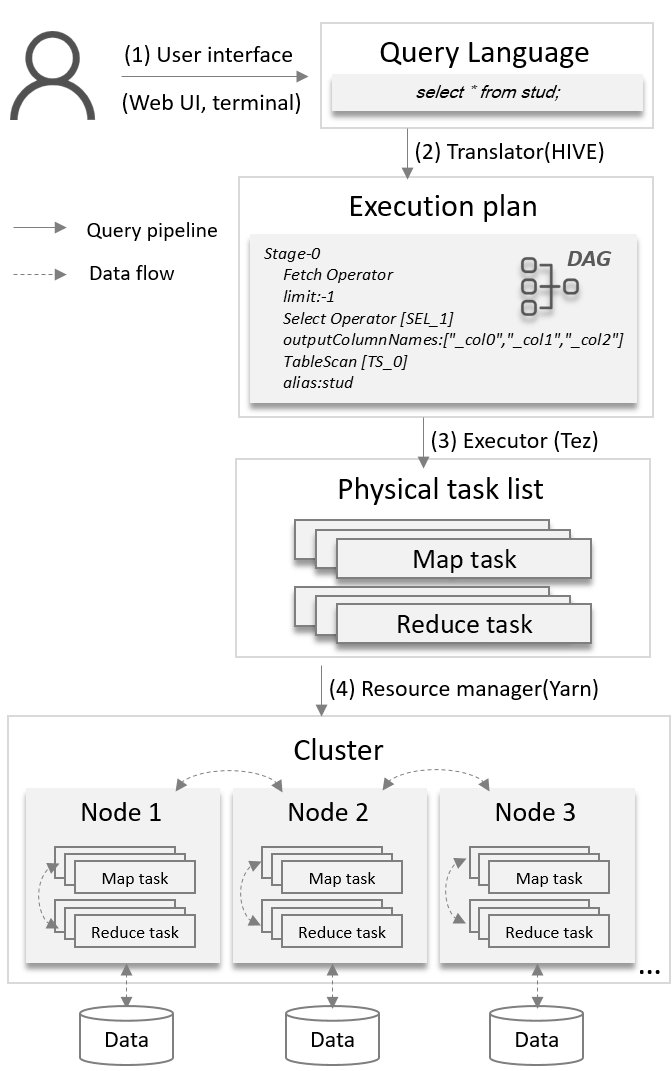
\includegraphics[width=0.48\textwidth]{figures/background/arc.png}
	\vspace{-3mm}
	\caption{Overview of distributed query pipeline(Hadoop 2.0).}
	\label{fig:architecture}
	\vspace{-3mm}
\end{figure}


% \begin{figure}[t]
% 	\centering
% 	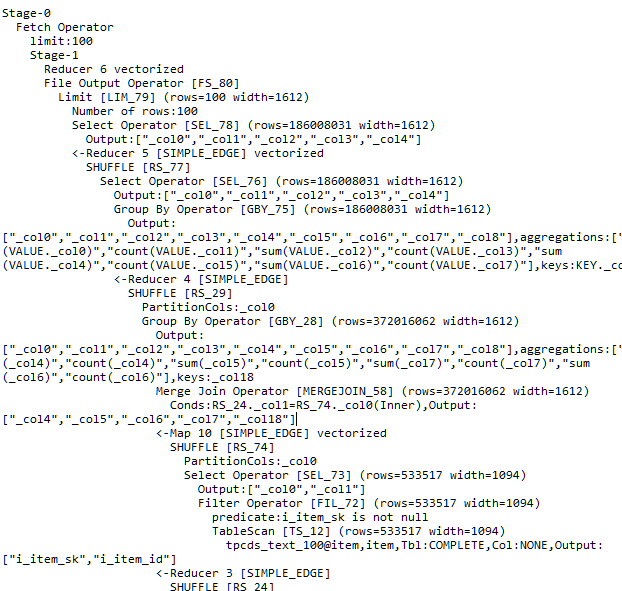
\includegraphics[width=0.45\textwidth]{figures/background/execution_plan.png}
% 	\vspace{-3mm}
% 	\caption{The hive execution plan.}
% 	\label{fig:exec_plan}
% 	\vspace{-3mm}
% \end{figure}

When user issues a query (shown as Figure~\ref{fig:architecture}(1)) through the interface such as a web-based user interface or SQL terminal. 
Hive uses a cost-based optimizer to optimize the query such as determining the best methods for scan operators, join orders and aggregate operation, and then translate it as the logic execution plan shown as Figure~\ref{fig:architecture}(2). The logic exaction plan may contains hundreds of lines of description, which describes the execution process as a Directed Acyclic Graph(DAG) that can be processed by the executor Tez. 

A DAG is a collection of vertices and edges. Logically, a \textbf{vertex} consists of a sequence of logical operators(such as filter, aggregate, etc) which describes the execution of a part of the query. Further more, there are two types of vertices in the Tez DAG, \textbf{map} vertex and reduce \textbf{vertex}. 
An \textbf{edge} defines the data movement of two adjacent vertices. We name of source vertex as the \textbf{producer} vertex and the target vertex as the \textbf{consumer} vertex. Noticed that a producer vertex may connect to multiple consumer vertices and a consumer vertex could be connected by multiple producer vertices.  

With a given vertex, Tez further creates a set of physical \textbf{tasks}(shown as Figure~\ref{fig:architecture}(3)). Then these tasks will be dispatched on the Hadoop machines by Yarn, the resource manage tool of Hadoop2.0. A task takes a piece of data as input and execute all operators  defined in the corresponding vertex. To ease the analysis of tasks, we define the sub-processes of a task as five steps. For a map task, the steps are \textit{Initialization}, \textit{Input}, \textit{Processor}, \textit{Sink}, \textit{Spill}. For a reduce task, the second step is \textit{Shuffle} instead. Moreover, the data read by a task could come from the local file or producer tasks.

\subsection{Requirement analysis}
During the one year of collaboration, we have closely collaborated with three experts in distributed database, who are also the co-authors of this paper.

In the first month of the collaboration, we have held brainstorming to collect the most frequent raised questions when analyzing the distributed query system performance. Based the discussions with domain experts and review of existing literature, we have formulated the following design requirements.

\begin{itemize}
  \item[\textbf{R1}]\textbf{Understand the general query execution trace and query plan structure.} Before our collaboration, the domain experts have used profiling software (TezVIS, etc) or visualization tools(Tableau, etc) to show the query progress as Ganntt chart and query plan structure as directed graph. However, these two visualizations are always displayed in separated views which require users to switch their focus and break the continuity of exploration.
  \item[\textbf{R2}]{Understand the query process at the task level.}Understand the execution of single task can be helpful to identify the bottleneck of the whole query process.However, visualize the tasks is challenge. First, to visualize the tasks in traditional way(Gantt diagram) need a large canvas. The multiple features such as the size of data and the operators should be visualized for understanding the task. Moreover, the many to many relationship among the tasks also makes it difficult to design clear and \textbf{scaleble} visualization.
  \item[\textbf{R3}]{Provide the visual insight to reason the behaviour and pattern of a specific task.}To solely visualize the tasks themselves are not enough to explain the specific pattern of tasks. Many reason about the hardware resource such as the network status, hard disk waiting list is also related to the patterns. Such kinds of information should be vitalized effectively to assist the exploration of query executions. 
  \item[\textbf{R4}]{ Support interactive exploration.} Other than the visualization designs, a flexible interaction should be implemented for users to navigate to any point of interest. The linkage among the correlated visual elements are also should be designed to coordinate the information.

\end{itemize}

\subsection{Task analysis}
Guided by the aforementioned requirements, we discussed with the domain experts about the visualization form and distilled the following visualization tasks:

\begin{itemize}
  \item[\textbf{T1}]\textbf{Visualize the execution process and query plan structure effectively.} To guarantee the continuity of exploration(R1), the process and plan structure should be integrated into one visualization view. Several criteria should be considered such as the minimize usage of canvas, minimize the cross of links and provide clear topology structure.
  \item[\textbf{T2}]\textbf{Effectively visualize the information of tasks.} To facilitate the fine grained exploration of query execution(\textbf{R1}, \textbf{R2}), the information about the tasks should be visualized, including: the size of data processed by the task; the data-flow among the tasks; the temporal information of task(start the time, end time, time usage, etc) and the corresponding sub-process. Moreover, the abnormal(tasks taking longer time) tasks should be easily observed.
  \item[\textbf{T3}]\textbf{Visualize the machine status.} Display the machine status such as network status, disk IO pending list, CPU usage and Memory Usage will be useful to investigate the characters of task, and reasoning the patterns of the query execution( \textbf{R3}).
  \item[\textbf{T4}]\textbf{Interaction and linkage.} System should provide the flexible interactions allowing users to switch the focus among the different point of interest, such as a specific time range, a vertex or a group of tasks(\textbf{R1}, \textbf{R2}, \textbf{R3}, \textbf{R4}). For example, user may select a vertex and explore if the tasks in this vertex are CPU-bound or I/O-bound. This requires the visualization to show the related tasks when choosing a vertex and highlight the corresponding CPU and dist information simultaneously.


\end{itemize}
